%!TEX root = ../main.tex

\section{Setup}
\label{sec:setup}

The experiment consists of several components. A schematic setup can be seen in 
\autoref{fig:setup}. An interferometer monitors the velocity at which the Mössbauer 
driving unit (MDU) as well as $\gamma$-source are moving relative to the lab frame.
An absorber can be placed in the beam path of the high-energy photons. Based on their
energy, the $\gamma$'s are either transmitted or absorbed by the target. The number 
of transmitted photons is counted by a 1024 channel multi-channel-scaler (MCS). The 
various other components of the setup (DFG, etc.) are used for calibration as 
well as data acquisition (DAQ) purposes, more detailed information on the individual
building blocks can be taken from \cite{Sch17}.

\begin{figure}[h]
	\centering
	\label{fig:setup}
	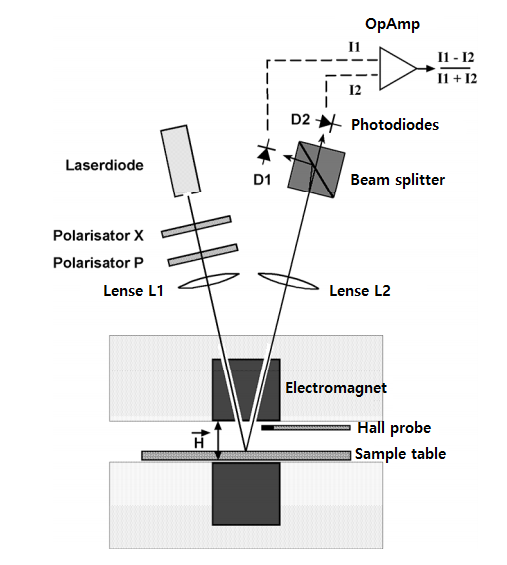
\includegraphics[width=0.7\textwidth]{./fig/setup.png}
	\caption{A schematic overview of the experiment components. The Mössbauer 
	driving unit (MDU) moves the $\gamma$-source at a velocity relative to the 
	multi-channel-scaler (MCS). The exact velocity can be controlled via a 
	digital function generator (DFG), Mössbauer velocity transducer (MVC) and 
	monitored by an interferometer.}
\end{figure}
